\documentclass[12pt,halfline,a4paper]{ouparticle}

\usepackage{booktabs}
\usepackage{xcolor}
\usepackage{graphicx}
\usepackage{caption}
\usepackage{subcaption}

\usepackage{cite}  % citeパッケージのインポート
\usepackage{natbib}  % 必要に応じて引用パッケージを使用


\begin{document}

\title{Does the Gender Employment Gap Expand Due to Natural Disasters? Evidence from the Great East Japan Earthquake\break {}}

\author{%
\name{Tomoto Masuda}
\address{}}

\abstract{This study analyzes the impact of the Great East Japan Earthquake of March 2011 on the gender employment gap in Fukushima Prefecture. Employing an event study approach alongside a difference-in-differences (DID) methodology with fixed effects regression, this study examines the earthquake's influence on gender-based employment dynamics. Drawing on extensive prefectural economic statistical data and individual socio-economic attributes from sources such as the Japan General Social Survey (JGSS), the Open Survey Data Japan Household Panel Survey on Consumer Preferences and Satisfaction (JHPS-CPS), the National Census, and the Housing and Land Survey, this study assesses the long-term effects of the earthquake on the gender employment gap. {\color{red}The results indicate that, in contrast to the immediate aftermath, the long-term impacts on the gender employment gap have attenuated significantly. This convergence can be primarily attributed to two factors: persistent governmental initiatives aimed at promoting female labor force participation, and the economically rational adaptations of households in response to disruptions in community structures.}}

\date{\today}

\keywords{word1; word2; word3; and word4}

\maketitle

\tableofcontents

\section{Introduction}
\label{sec1}

How does a natural disaster impact gender disparities within the labor markets of the affected regions? Previous studies present mixed findings on the impact of natural disasters on gender inequality, with some research indicating that such disasters widen gender gaps while other studies suggest a narrowing of these gaps. The Great East Japan Earthquake of March 2011 presented a unique opportunity to examine the dynamics of labor market responses to significant external shocks. This study focuses on Fukushima Prefecture, an area profoundly affected by both the earthquake and subsequent nuclear incident, to analyze the short-term and long-term impacts on the gender employment gap.


To frame the analysis, this study employs a comprehensive theoretical household model that encompasses four key elements. First, this study considers household decision-making processes, where utility maximization drives choices about labor supply and participation. This model recognizes that households make complex decisions balancing immediate needs with long-term economic rationality, often leading to gendered patterns of labor market engagement.

Secondly, the model incorporates the concept of economic shocks and adaptation mechanisms. The immediate aftermath of the disaster likely triggered rapid changes in employment patterns. However, over time, households develop adaptation strategies, including adjustments in labor supply preferences, acquisition of new skills, and reallocation of household labor responsibilities.

Thirdly, this study acknowledges the crucial role of government policies in shaping labor market outcomes. The theoretical framework examines how interventions aimed at promoting gender equality in employment can mitigate the adverse effects of economic shocks. This study assesses the effectiveness of these policies in both the short and long term, recognizing that policy impacts may evolve over time.

Lastly, the model considers the impact of community structure on household decision-making. The earthquake and its aftermath significantly disrupted local infrastructure and social networks, potentially altering the context in which households make employment decisions. We posit that long-term community rebuilding efforts can influence labor market dynamics and potentially reshape gender roles within households and the broader community.

By integrating these four elements - household decision-making, economic shocks and adaptation, policy interventions, and community structure - our theoretical model provides a comprehensive framework for understanding the complex interplay of factors affecting the gender employment gap in the wake of a major disaster. This study aims to contribute to the broader literature on labor market resilience and gender dynamics in employment, offering insights that may be applicable to other contexts of significant economic disruption.



ジェンダー固有の影響とその経済的なメカニズムについて詳細に論じる。



This paper explores the mechanisms through which the Great East Japan Earthquake impacted gender employment gaps for men and women as follows: First, in the short-term immediately after the disaster, women's employment decreased more than men's, widening the gender gap. This can be attributed to the higher prevalence of non-regular employment among women compared to men, as well as women's role as risk buffers for household adjustments. However, in the longer run, women's employment recovered rapidly, narrowing the gender gap. This reversal can be explained by two factors: a delayed onset of government policies promoting women's employment opportunities, and previously non-employed women (engaged in domestic labor or assisting family businesses) entering the labor force to supplement household income in the aftermath of the earthquake.


“The ‘Act on Promotion of Women’s Participation and Advancement in the Workplace’ enacted in April 2016 has led to the development of an environment conducive to working women of child-rearing generations, with initiatives such as the introduction of a reduced working hours system, restrictions on overtime work, and the establishment of childcare facilities within companies.”


2016年4月に施行された「女性活躍推進法」により、短時間勤務制度や所定外労働の制限、託児所の社内設置など、子育て世代の女性が働きやすい環境づくりが進められた。

This paper presents theoretical household model to explain...




\begin{figure}
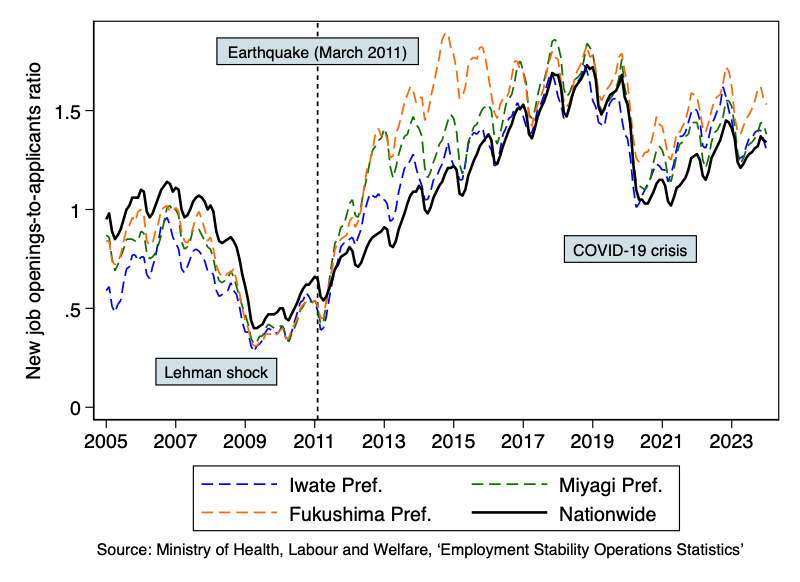
\includegraphics[width=\textwidth]{New job openings-to-applicants ratio.png}
\caption{New job openings-to-applicants ratio} \label{New job openings-to-applicants ratio.png}
\end{figure}


Public employment security office 

\begin{figure}
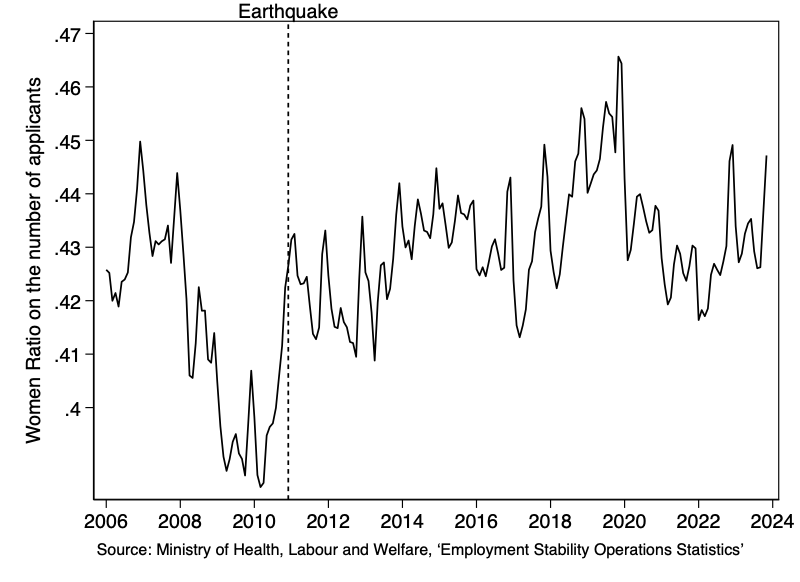
\includegraphics[width=\textwidth]{Women ratio on the number of applicants in Fukushima.png}
\caption{Women ratio on the number of applicants in Fukushima Pref.} \label{Women ratio on the number of applicants in Fukushima.png}
\end{figure}



\begin{figure}
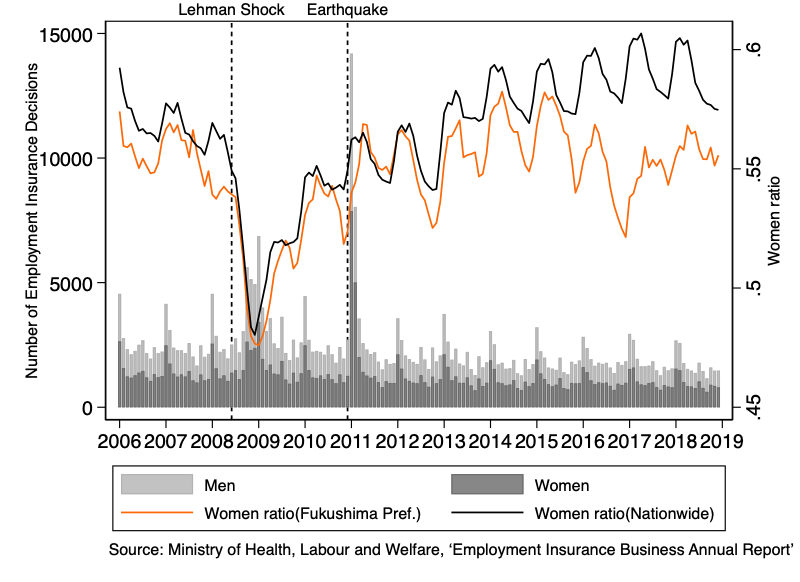
\includegraphics[width=\textwidth]{Number of Employment Insurance Decisions_2.png}
\caption{Number of Employment Insurance Decisions by gender in Fukushima Pref.} \label{Number of Employment Insurance Decisions_2.png}
\end{figure}


\section{Background}
\label{sec2}

\subsection{The Great East Japan Earthquake }
\label{sec5.1}

The Great East Japan Earthquake of March 2011 resulted in a tripartite catastrophe, comprising a magnitude 9.0 earthquake, a devastating tsunami, and a nuclear accident at the Fukushima Dai-ichi Nuclear Power plant. This disaster precipitated a severe humanitarian crisis, causing extensive damage particularly in the Iwate, Miyagi, and Fukushima prefectures in northeast Japan. According to the National Police Agency, 15,900 people lost their lives and 2,523 people remain unaccounted for, primarily as a result of the
massive tsunami that struck the eastern coast of Japan. The affected
prefectures account for 99.6\% of total fatalities and 99.8\% of total missing persons. In addition, a total of 3,784 fatalities and casualties were recognized as disaster-related deaths in Japan due to the exacerbation of chronic illnesses or suicide during evacuation. Approximately 90\% of fatalities were attributed to drowning. Table 1 presents a summary of the damages in the affected prefectures. The map below indicates the epicenter of the earthquake.

\begin{flushleft}
\begin{table}[h!]
  \caption{Direct Impact Overview in the Disaster-Stricken Prefectures}\label{table:disaster_situation}
  \begin{minipage}[c]{0.4\textwidth}
    \includegraphics[width=\textwidth,height=1.10\textwidth]{epicenter.jpeg}
  \end{minipage}
  \begin{minipage}[c]{0.48\textwidth}
    \raggedright
    \scalebox{0.8}{
    \begin{tabular}{|c|c|c|c|}
    \hline
    & \multicolumn{1}{c|}{Iwate} & \multicolumn{1}{c|}{Miyagi} & \multicolumn{1}{c|}{Fukushima} \\
    \hline
    Population & 1,330,147 & 2,348,165 & 2,029,064 \\
    Deceased & 4,675 & 9,544 & 1,614 \\
    Missing & 1,110 & 1,213 & 196 \\
    Fully destroyed houses & 20,185 & 83,932 & 20,136 \\
    Partially destroyed houses & 4,562 & 138,721 & 65,093 \\
    \hline
    \end{tabular}
    }
  \end{minipage}
\end{table}
\end{flushleft}

Fukushima Prefecture experienced a compound disaster involving both the tsunami triggered by the earthquake and the subsequent nuclear accident. The nuclear incident, in particular, necessitated large-scale evacuations, significantly disrupting local communities and labor markets. This unprecedented situation provides a unique context for examining the long-term socioeconomic impacts of compound disasters.


\subsection{Gender Gap in Japan}
\label{sec5.1}

According to the latest 2024 Global Gender Gap Report by the World Economic Forum (WEF), Japan ranks 118th out of 146 countries, placing it at the bottom among the G7 nations. Particularly, its rankings in the "Economic" and "Political" domains are notably low, with the "Economic" ranking being 120th out of 146 countries. Japan continues to exhibit substantial gender disparities in the economic sector, with the elimination of wage gaps remaining a significant challenge.

\section{Data and Descriptive Statistics}
\label{sec4}

This study utilizes the exogeneity of the impact of the Great East Japan Earthquake to conduct a regression analysis. 

\subsection{DATA}
\label{sec5.1}

The main data used in the paper is Open Survey Data Japan Household Panel Survey on Consumer Preferences and Satisfaction (JHPS-CPS) collected by Osaka University under the 21st Century COE Program.


\section{Literature review}
\label{sec3}



Development economics models suggest an increase in household members’ labour supply as a shock-coping strategy which is associated with the narrowing of gender employment gaps. Several studies have documented a rise in female labor force participation following natural disasters. For instance, Canessa and Giannelli (2021)\cite{Canessa2021WomensShocks} examine the impact of severe flooding in Bangladesh on women's employment and empowerment using georeferenced and longitudinal household panel data. Their difference-in-differences analysis reveals a significant 13 percentage point increase in women's employment probability post-flood. 


On the other hand, in labor economics, the Risk Adjustment Hypothesis posits that during economic shocks or natural disasters, women are more susceptible to labor market exclusion and face higher risks of deteriorating work conditions or unemployment compared to men. This hypothesis suggests that specific labor market subgroups, particularly female and non-regular workers, often function as 'adjustment valves,' absorbing economic shocks. These groups are disproportionately affected, serving as mechanisms to mitigate broader economic impacts. This framework illuminates the gender-based disparities in employment stability and the uneven distribution of economic resilience across worker categories during crises. For instance, Kim, Ashley, and Corcoran (2014) examines the economic impact of the 2010 earthquake in Haiti, focusing on changes in household composition and employment retention. Authors found that the earthquake caused a significant reduction in employment rates, from 52.6\% prior to the earthquake to 28.6\% five months post-event. Gender disparities were evident, with only 34.2\% of women retaining their employment compared to 55.6\% of men. 


The study tries to fill gaps in the still sparse literature on the impact of natural disasters on gender disparities by differentiating between short-term and long-term effects, addressing the contradictory findings of existing research that suggests either an exacerbation or a reduction of gender gaps.


\section{Results}
\label{sec5}

\subsection{Results}
\label{sec5.1}


Initially, these events disproportionately impacted women workers negatively. However, The earthquake and nuclear disaster potentially accelerated women's labor market participation by fundamentally disrupting communities bound by traditional gender roles. In the short term, the disaster and nuclear accident had a more severe negative impact on female workers. However, in the long term, this catastrophic event, while devastating, may have inadvertently challenged long-standing societal norms, thus facilitating increased female workforce engagement.


% すべての文献を引用リストに追加
\nocite{*}

% 参考文献リストの場所を示す
\bibliography{references}  % 'references.bib'ファイルの名前を指定
\bibliographystyle{plain}  % 引用スタイルを指定


\end{document}
